
%----------------------------------------------------------------------------------------
%	PACKAGES AND OTHER DOCUMENT CONFIGURATIONS
%----------------------------------------------------------------------------------------

\documentclass[paper=a4, fontsize=11pt]{scrartcl} % A4 paper and 11pt font size

\usepackage[T1]{fontenc} % Use 8-bit encoding that has 256 glyphs
\usepackage{fourier} % Use the Adobe Utopia font for the document - comment this line to return to the LaTeX default
\usepackage[english]{babel} % English language/hyphenation
\usepackage{amsmath,amsfonts,amsthm} % Math packages

\usepackage{lipsum} % Used for inserting dummy 'Lorem ipsum' text into the template

\usepackage{sectsty} % Allows customizing section commands
\allsectionsfont{\centering \normalfont\scshape} % Make all sections centered, the default font and small caps
\usepackage{amsfonts}
\usepackage[utf8]{inputenc}
\usepackage[margin=1in]{geometry}
\usepackage{hyperref}
\usepackage{amssymb, latexsym}
\usepackage{amsmath}
\usepackage{listings}
\usepackage{graphicx}
\usepackage{fancyhdr} % Custom headers and footers
\pagestyle{fancyplain} % Makes all pages in the document conform to the custom headers and footers
\fancyhead{} % No page header - if you want one, create it in the same way as the footers below
\fancyfoot[L]{} % Empty left footer
\fancyfoot[C]{} % Empty center footer
\fancyfoot[R]{\thepage} % Page numbering for right footer
\renewcommand{\headrulewidth}{0pt} % Remove header underlines
\renewcommand{\footrulewidth}{0pt} % Remove footer underlines
\setlength{\headheight}{13.6pt} % Customize the height of the header

\numberwithin{equation}{section} % Number equations within sections (i.e. 1.1, 1.2, 2.1, 2.2 instead of 1, 2, 3, 4)
\numberwithin{figure}{section} % Number figures within sections (i.e. 1.1, 1.2, 2.1, 2.2 instead of 1, 2, 3, 4)
\numberwithin{table}{section} % Number tables within sections (i.e. 1.1, 1.2, 2.1, 2.2 instead of 1, 2, 3, 4)

\setlength\parindent{0pt} % Removes all indentation from paragraphs - comment this line for an assignment with lots of text

%----------------------------------------------------------------------------------------
%	TITLE SECTION
%----------------------------------------------------------------------------------------

\newcommand{\horrule}[1]{\rule{\linewidth}{#1}} % Create horizontal rule command with 1 argument of height

\title{	
\normalfont \normalsize 
\textsc{UNIVERSITY OF CALIFORNIA, LOS ANGELES} \\ [25pt] % Your university, school and/or department name(s)
\horrule{0.5pt} \\[0.4cm] % Thin top horizontal rule
\huge STATS 202A Final Homework \\ % The assignment title
\horrule{2pt} \\[0.5cm] % Thick bottom horizontal rule
\author{Salil S. Kanetkar} % Your name
\normalsize{UID : 704557096}
\date{\normalsize\today} % Today's date or a custom date
}


\begin{document}
\maketitle% prints the title block
\textbf{Solution Problem 1:} \\
\textit{CPP Code:}
\begin{lstlisting}
#include <RcppArmadilloExtensions/sample.h>
//[[Rcpp::depends(RcppArmadillo)]]
using namespace Rcpp;
using namespace arma;

// [[Rcpp::export]]
arma::vec runifC(double seed, int n) 
{
  double x = seed;
  arma::vec u(n); 
  for(int i = 0; i < n; ++i)
  {                                      
    x = fmod(pow(7,5) * x, pow(2,31) - 1.0);
    u[i] = x / (pow(2,31) - 1.0);
  }
  return(u);
}

// [[Rcpp::export]]
arma::vec rnormC(double seed, int n) 
{
  double pi = 3.141592653589793238462643383280;
  double theta; 
  double r;
  arma::vec u(2);     
  arma::vec v(2 * n);
  for(int i = 0; i < n; ++i)
  {
    u = runifC(seed * (i + 1), 2);
    theta = 2.0 * pi * u[0];
    r = sqrt(-2 * log(u[1]));
    v[2 * i] = r * cos(theta);
    v[(2 * i) + 1] = r * sin(theta);
  }
  return(v);
}
\end{lstlisting}

\textit{R Code:}
\begin{lstlisting}
#For Uniform Generator
library(Rcpp)
sourceCpp("stats_final.cpp")
par(mfrow=c(1,2))
hist(runifC(12345, 10000), xlab ="U",prob=T,main="Histogram of U")
plot(runifC(12345, 10000)[seq(2,1000,by=2)], runifC(12345, 10000)[seq(3,1001,by=2)] , xlab = expression('x'[2*t]), ylab = expression('x'[2*t+1]), main="catterplot")

#For Normal Generator
hist(rnormC(76543, 10000),xlab="X and Y",main = "Histogram of X and Y", xlim =c(-4,4))
normal = rnormC(76543,10000)
x = normal[seq(1,20000,by=2)]
y = normal[seq(2,20000,by=2)]
par(mfrow =c(1,2))
hist(x , breaks =30, prob =T, xlim =c(-4,4) , xlab ="X", main = "Histogram of X")
curve(dnorm(x,mean =0, sd =1) ,lwd =2, add =T, col="blue")
hist(y , breaks =30, prob =T, xlim =c(-4,4), xlab ="Y", main = "Histogram of Y")
curve(dnorm(x,mean =0, sd =1) ,lwd =2, add =T, col="blue")

\end{lstlisting}


\begin{figure}[h!]
	\centering
	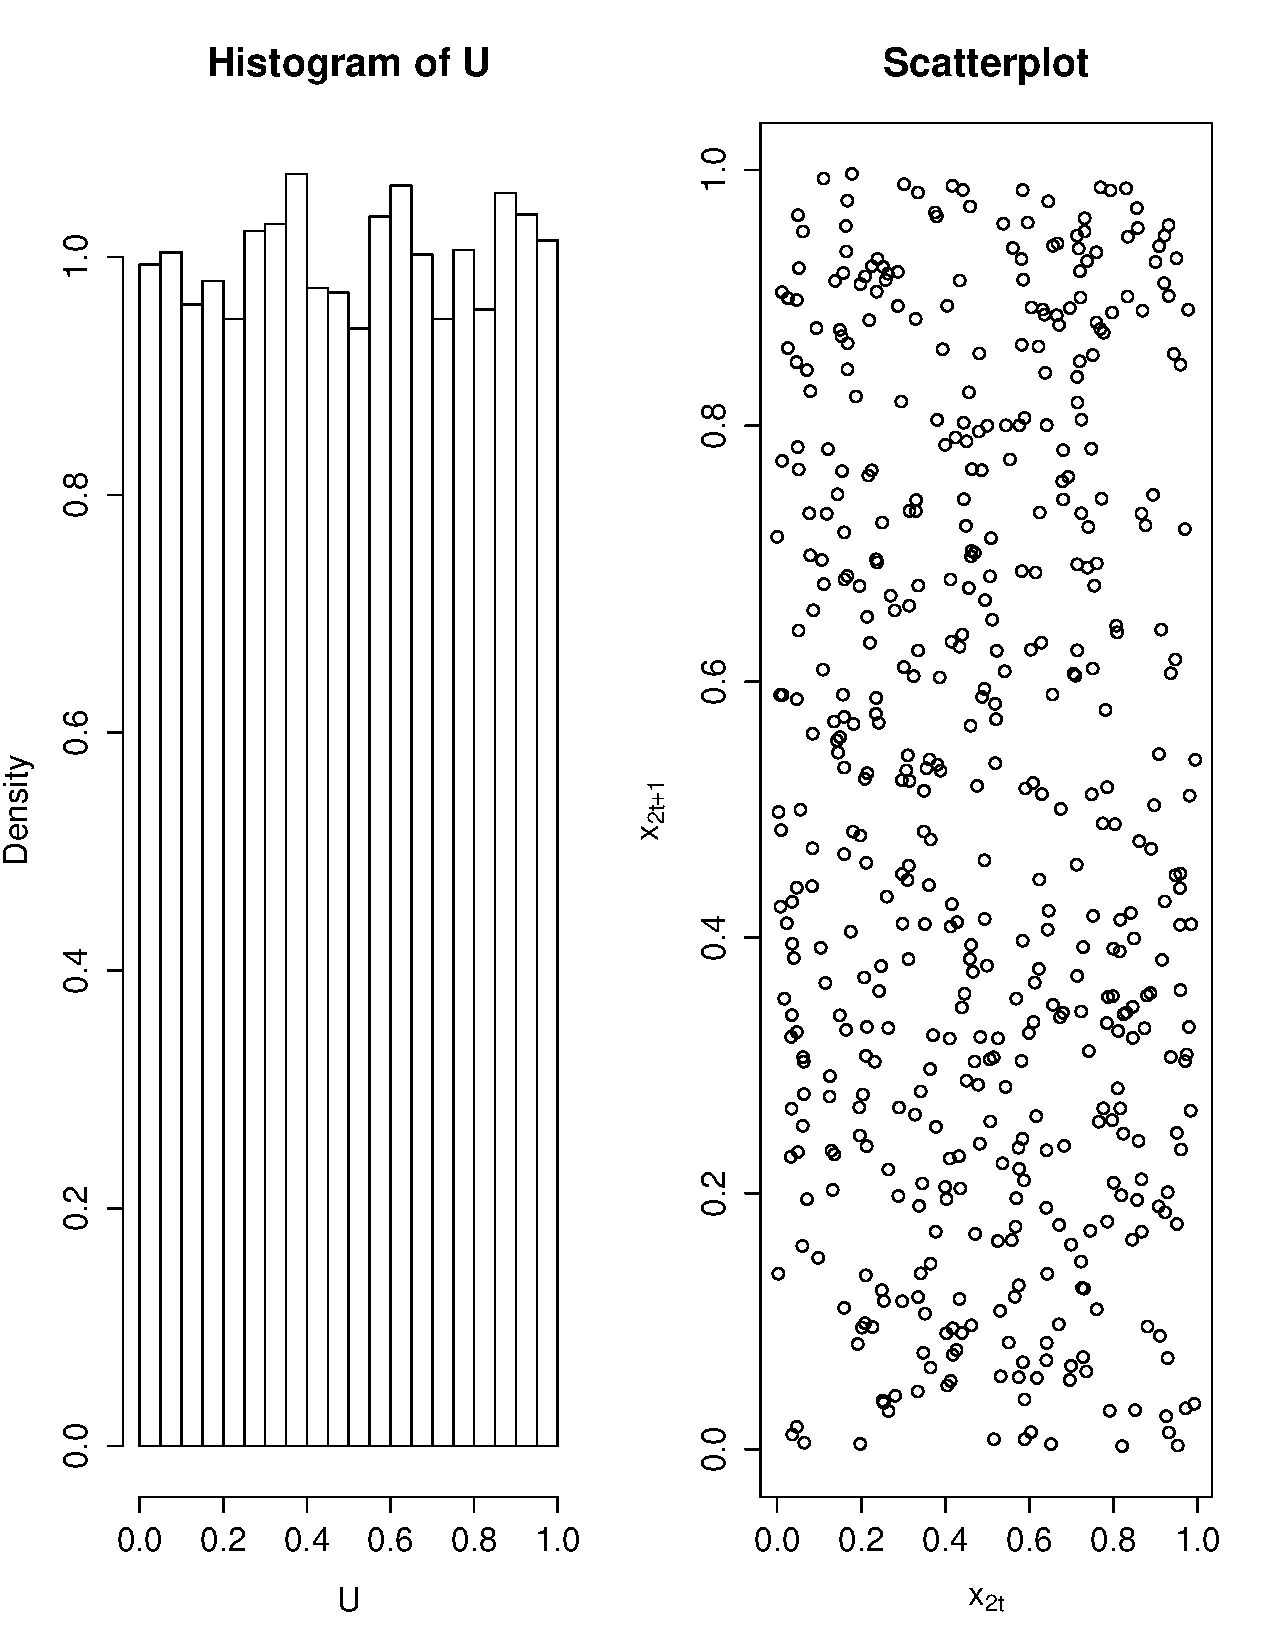
\includegraphics[width=15cm, height=10cm]{1a.pdf}
	\caption{Problem 1 - Uniform Distribution using Linear Congruential Method} 
\end{figure}

\begin{figure}[h!]
	\centering
	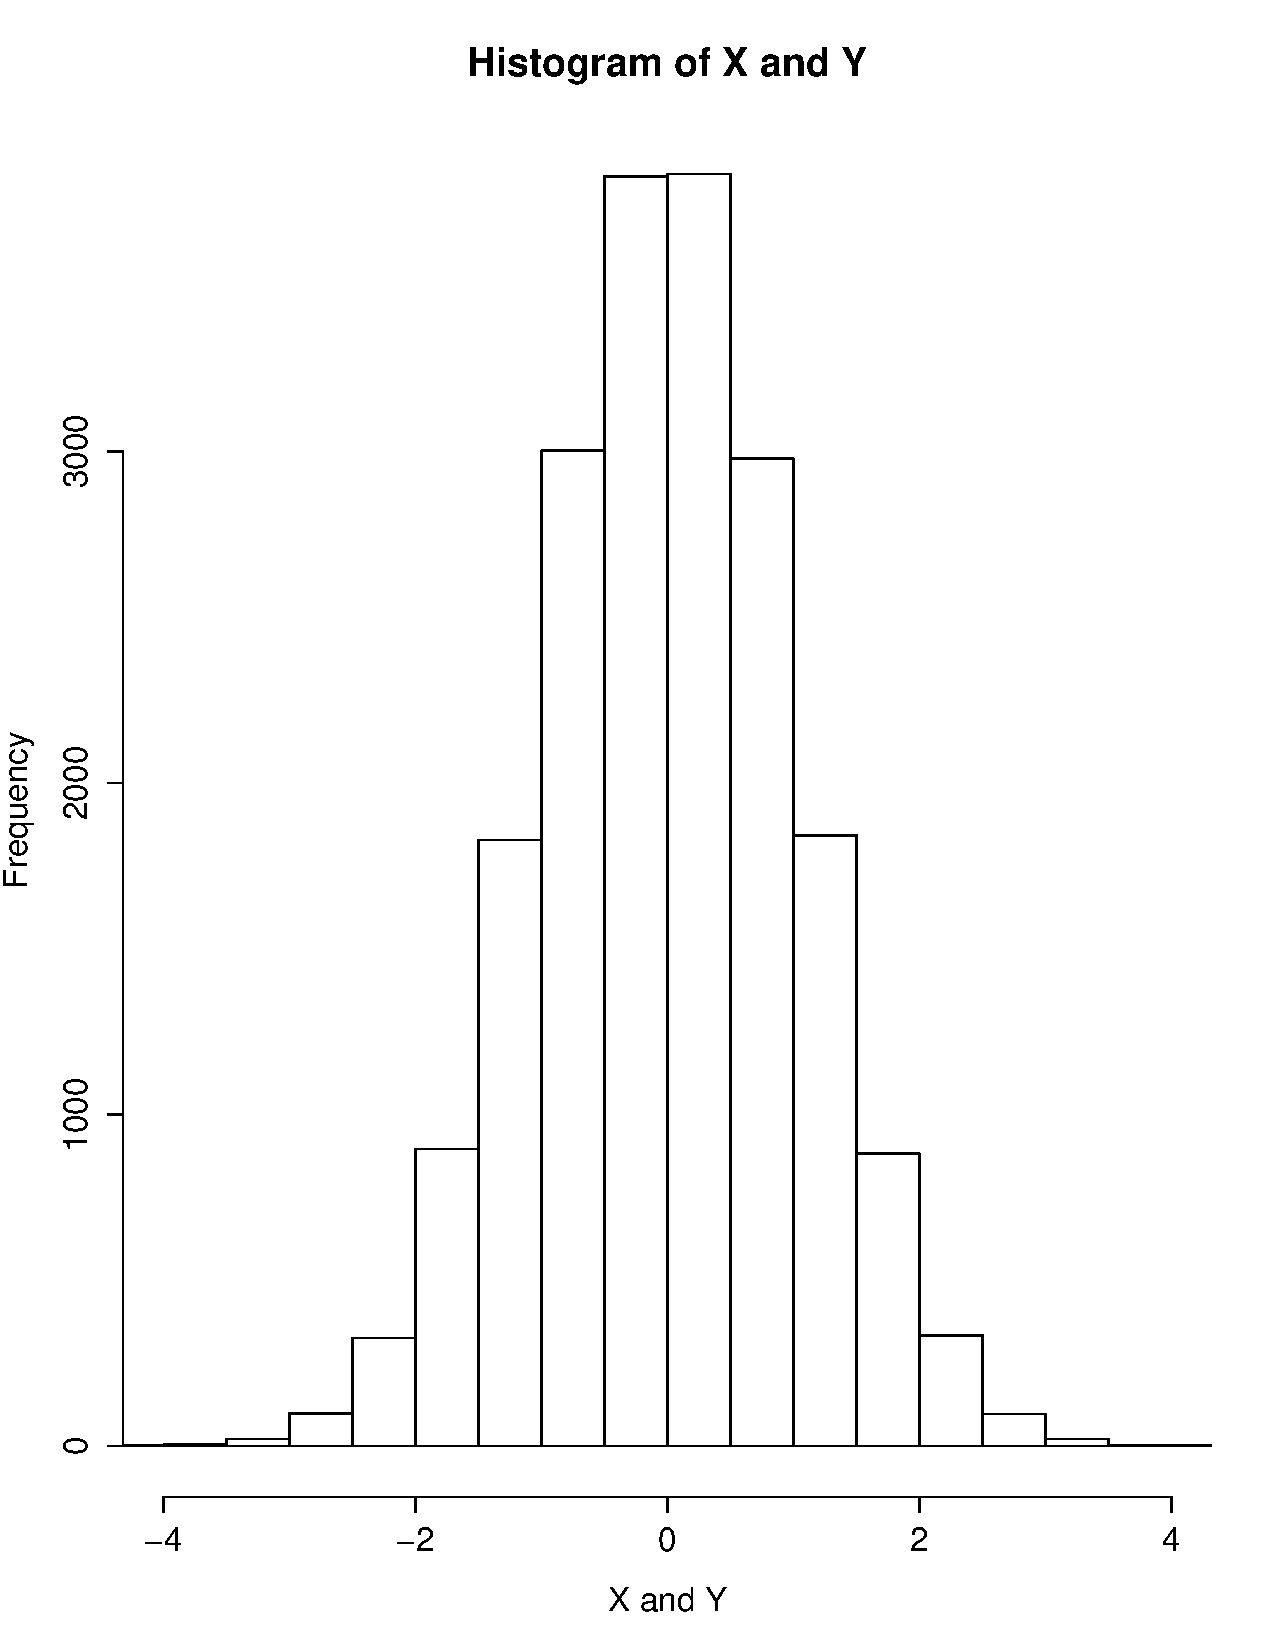
\includegraphics[width=15cm, height=10cm]{1ba.pdf}
	\caption{Problem 1 - Normal Distribution using Polar Transformation of X and Y} 
\end{figure}

\begin{figure}[h!]
	\centering
	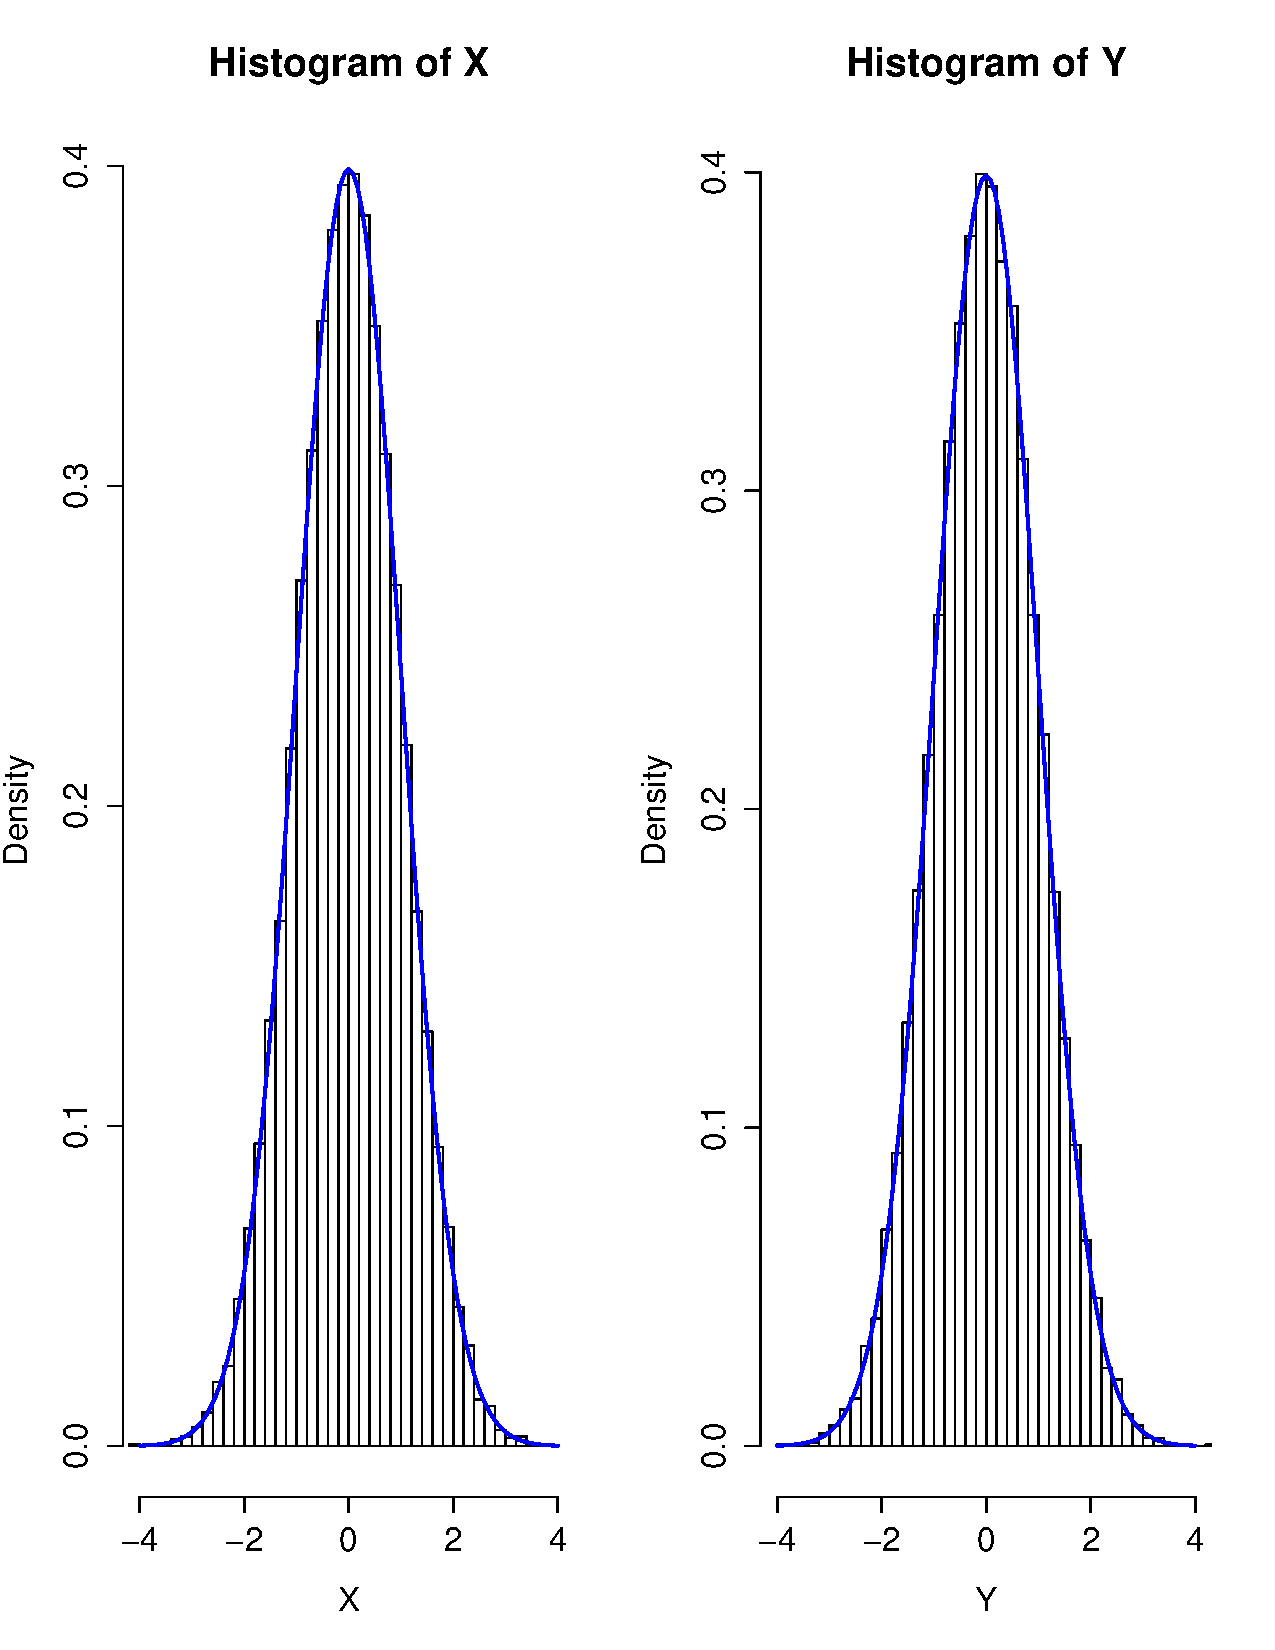
\includegraphics[width=15cm, height=10cm]{1bb.pdf}
	\caption{Problem 1 - Normal Distribution using Polar Transformation} 
\end{figure}

\clearpage

\textbf{Solution Problem 2:} \\
\textit{CPP Code:}

\begin{lstlisting}
#include <RcppArmadillo.h>
#include <RcppArmadilloExtensions/sample.h>
//[[Rcpp::depends(RcppArmadillo)]]
using namespace Rcpp;
using namespace arma;
// [[Rcpp::export]]
double f(long x, int variance)
{
  return (exp(-pow(x,2)/(2*variance)));
}

// [[Rcpp::export]]
double alpha(long x, long y, int variance = 2)
{
  return (1.0<(f(y,variance)/f(x,variance))) ? 1.0 : (f(y,variance)/f(x,variance));
}

// [[Rcpp::export]]
arma::vec metropolisCPP(arma::vec ch, long N, long T) 
{
  //arma::mat ch = clone(chain);
  long y;
  for(int n=0;n<N;n++)
  {
    long x=0;
    for(int i=0;i<T;i++)
    {
      arma::vec u1(10001);
      u1 = runifC(12345,10001);
      if(u1(n)>0.5)
      {
        y = x + 1;
      }
      else
      {
        y = x - 1;
      }
      arma::vec u2 = runifC(123,10001);
      int accept = (u2[n]<alpha(x,y));
      if(accept == 1)
      {
        x = y;
      }
      else
      {
        x = x;
      }
    }
    ch[n] = x;
  }
  return ch;
}
\end{lstlisting}

\textit{R Code:}

\begin{lstlisting}
library(Rcpp)
sourceCpp("stats_final.cpp")
N=10^3
T = 10^2
chain = matrix(0,1,N)
chain1 =  metropolisCPP(chain, N, T)
hist(chain1,xlim=range(c(-25,25)),freq=FALSE)
\end{lstlisting}

\begin{figure}[h!]
	\centering
	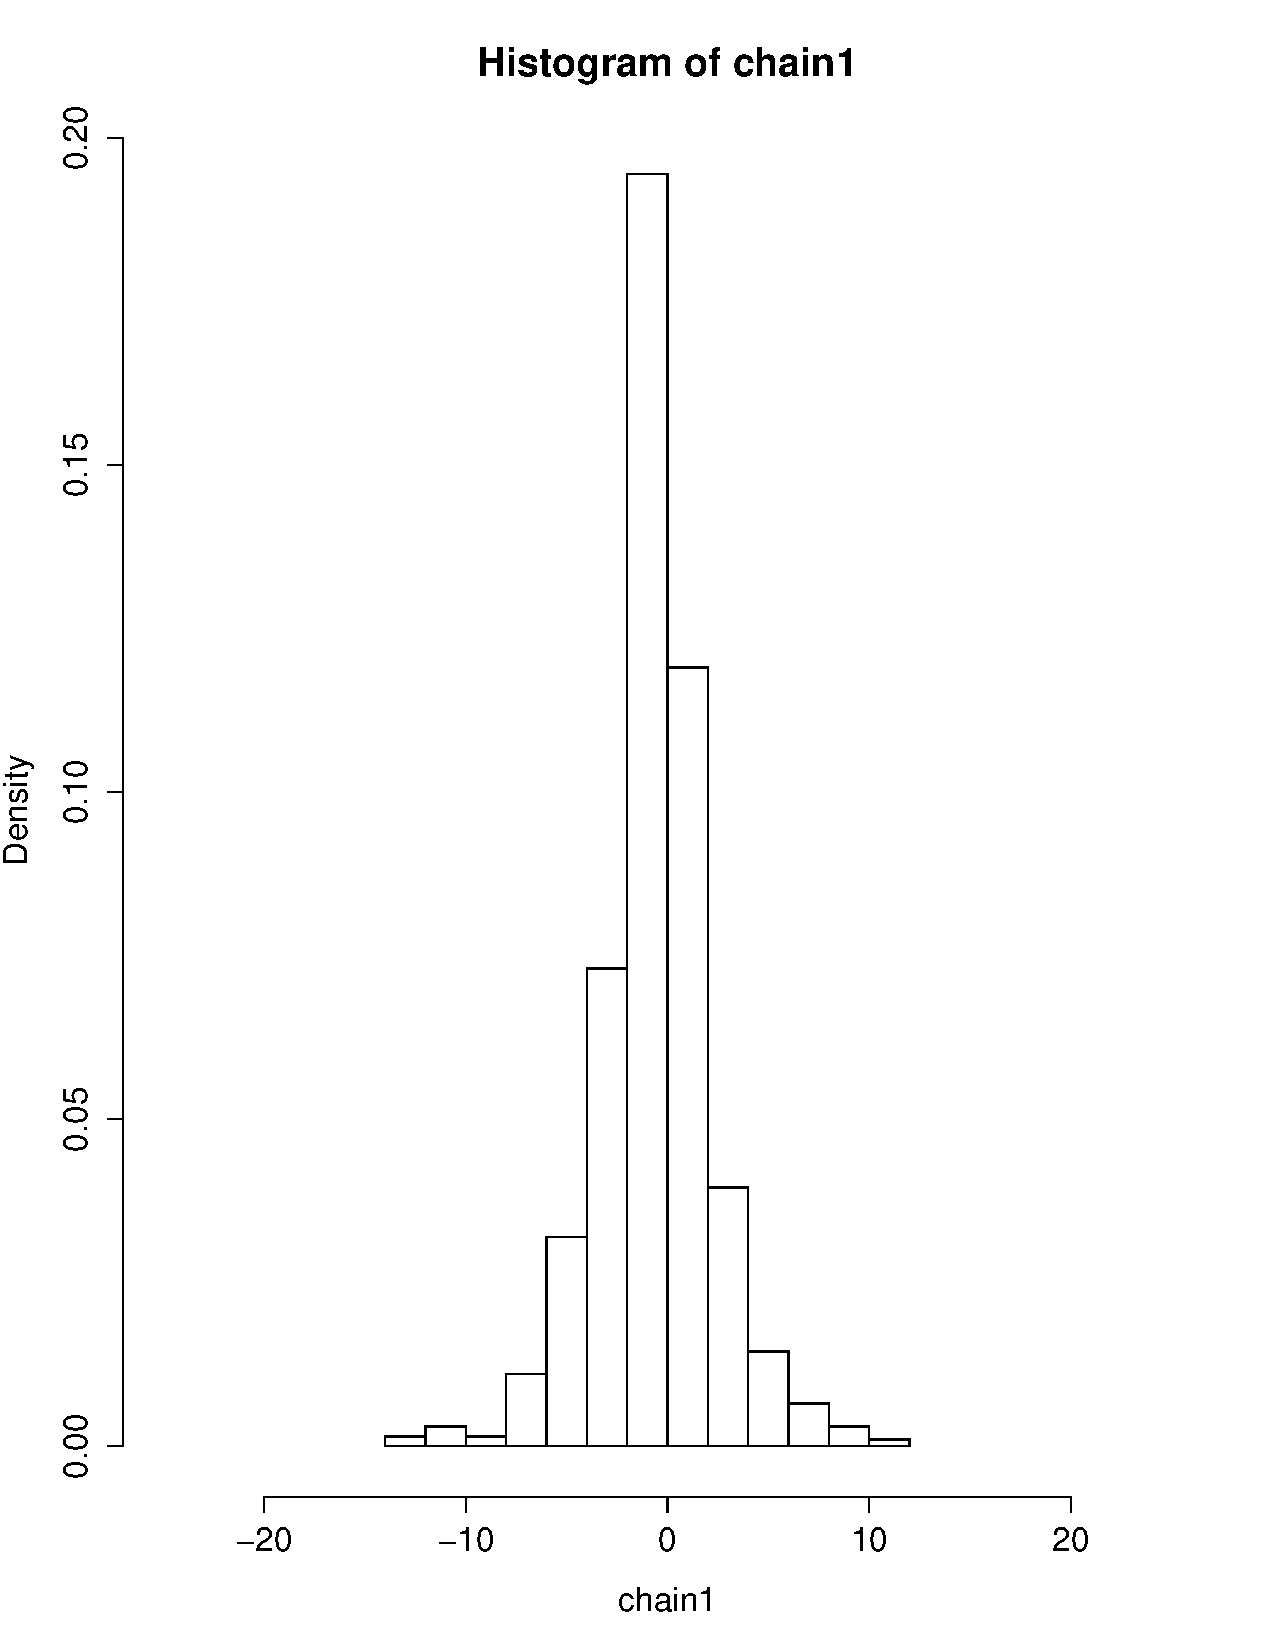
\includegraphics[scale = 0.5]{2.pdf}
	\caption{Problem 2 - Metropolis algorithm to sample from $\pi$} 
\end{figure}

\newpage
\textbf{Solution Problem 3:} \\
\textit{CPP Code:}

\begin{lstlisting}
#include <RcppArmadillo.h>
#include <RcppArmadilloExtensions/sample.h>
//[[Rcpp::depends(RcppArmadillo)]]
using namespace Rcpp;
using namespace arma;
// [[Rcpp::export]]
arma::cube gibbsCPP(NumericVector p2, int T, int M, double rho, double x0, double y0) 
{
  IntegerVector dim_p2=p2.attr("dim");
  arma::cube p(p2.begin(), dim_p2[0], dim_p2[1], dim_p2[2]);
  double x, y;
  arma::vec n1 = rnormC(76543,M*T);
  //arma::vec n2 = rnormC(76543,M*T);
  for(int m=0;m<M;m++)
  {
    x = x0;
    y = y0;
    p(0,0,m) = x;
    p(1,0,m) = y;
    for(int t=1;t<T;t++)
    {
      x = n1[m*T];
      x = x * sqrt(1-pow(rho,2)) + rho * y;
      y = n1[m*T+1];
      y = y * sqrt(1-pow(rho,2)) + rho * x;
      p(0,t,m) = x;
      p(1,t,m) = y; 
    }
  }
  return(p);
}
\end{lstlisting}

\textit{R Code:}

\begin{lstlisting}
library(Rcpp)
sourceCpp("stats_final.cpp")
gibbs<-function (T=1000, M=100, rho, x0, y0) 
{
  p<-rep(0,2*M*T) #Allocate memory for results
  dim(p)<-c(2,T,M)
  p1 = gibbsCPP(p,T=1000,M=100,rho,x0,y0) 
  p1
}

#making a movie
library(animation)
rho <- 0.99
M=100
par(mar=c(2,2,1,2), mfrow=c(3,3))
bvn <- gibbs(x0=-5,y0=0,M=M,rho=rho)
lims <- 8*c(-1,1)
for (t in 1:9){ plot(bvn[1,t,],bvn[2,t,],
                     xlim=lims, ylim=lims,
                     col=1:M,
                     pch=16, main=paste('t =',t))
  ani.pause(.2)
}#saving as GIF file
saveGIF({ for (t in 1:9){ plot(bvn[1,t,],bvn[2,t,], xlim = lims, ylim = lims, col=1:M,
                               pch =16, main = paste('t =',t))
}
}, movie.name =paste("bvn_gibbs_rho_", rho))
\end{lstlisting}

\textbf{Below are 3 figures obtained by varying the value of $\rho, X_0, Y_0$ }\\

\newpage
\begin{figure}[h!]
	\centering
	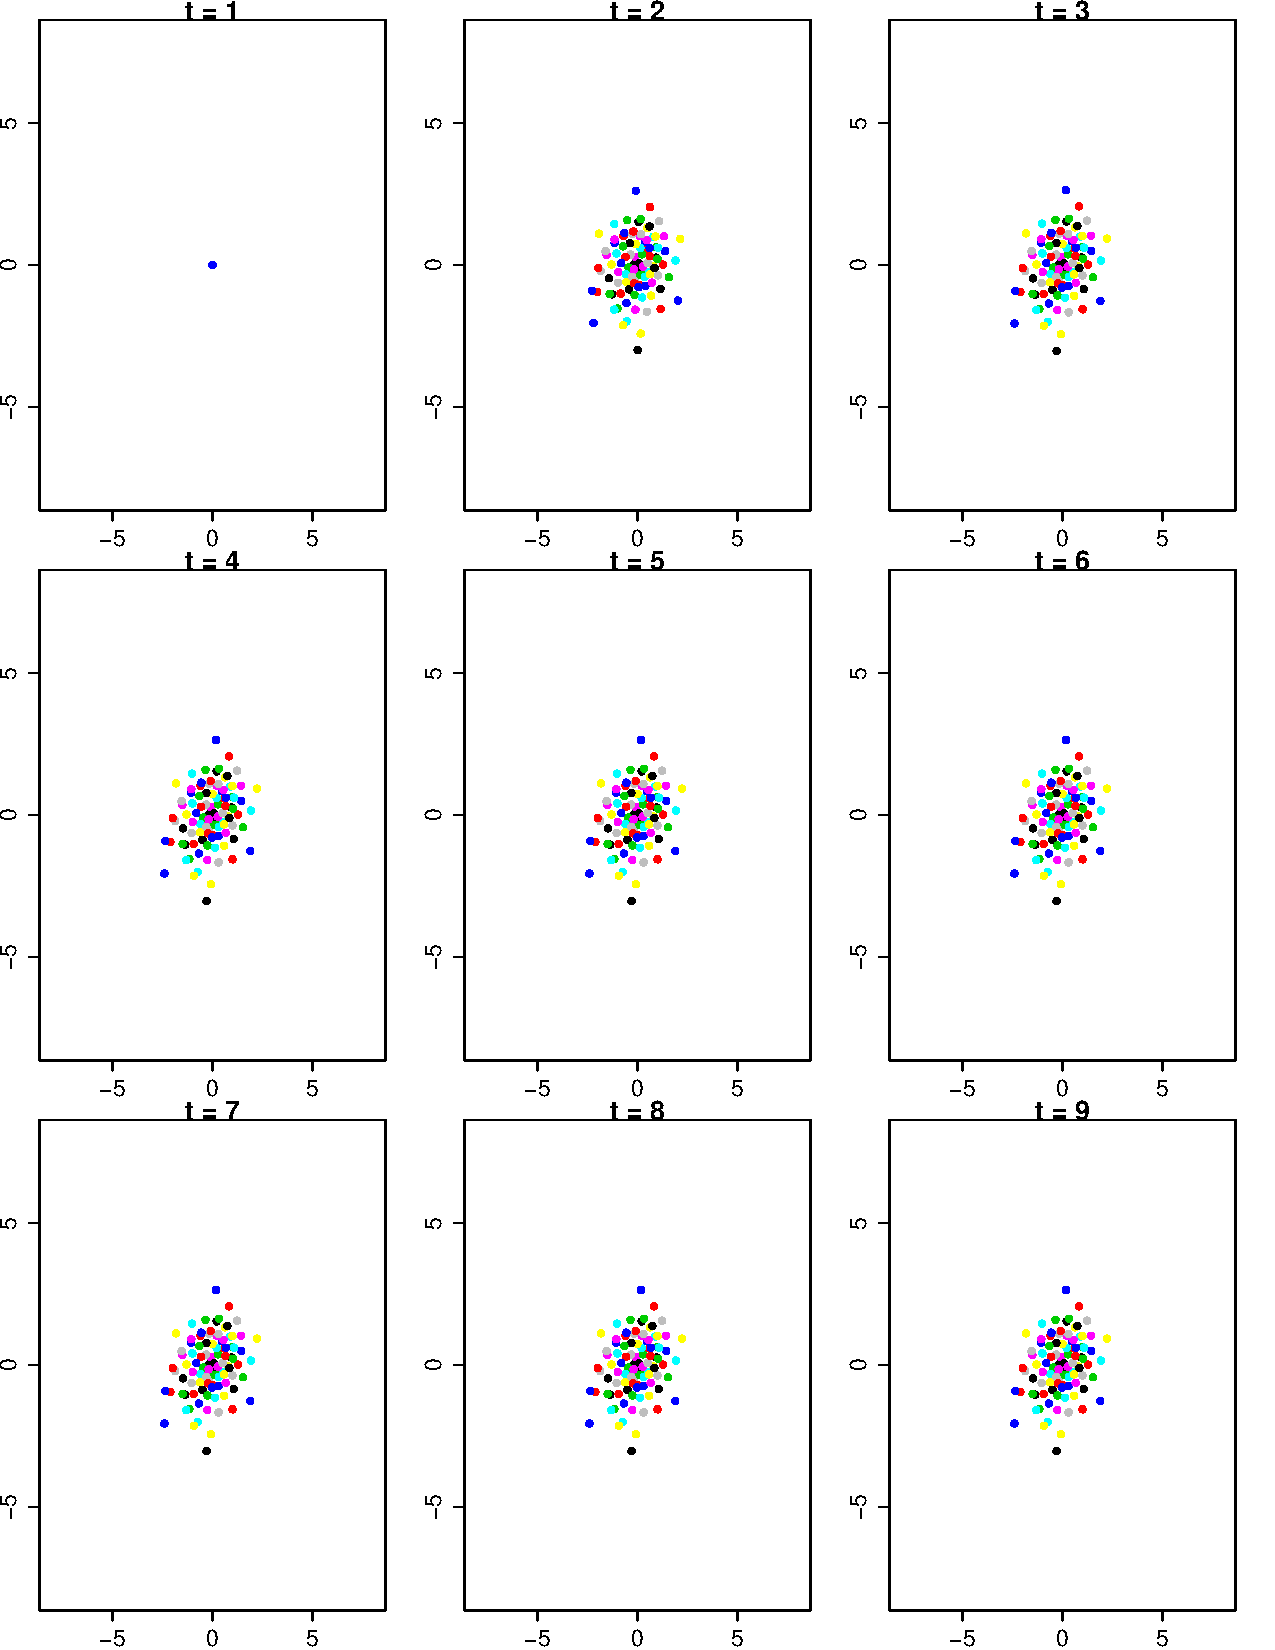
\includegraphics[scale = 0.8]{3a.pdf}
	\caption{Problem 3 - $X_0 = 0, Y_0 = 0, \rho = 0.1$} 
\end{figure}
\newpage
\begin{figure}[h!]
	\centering
	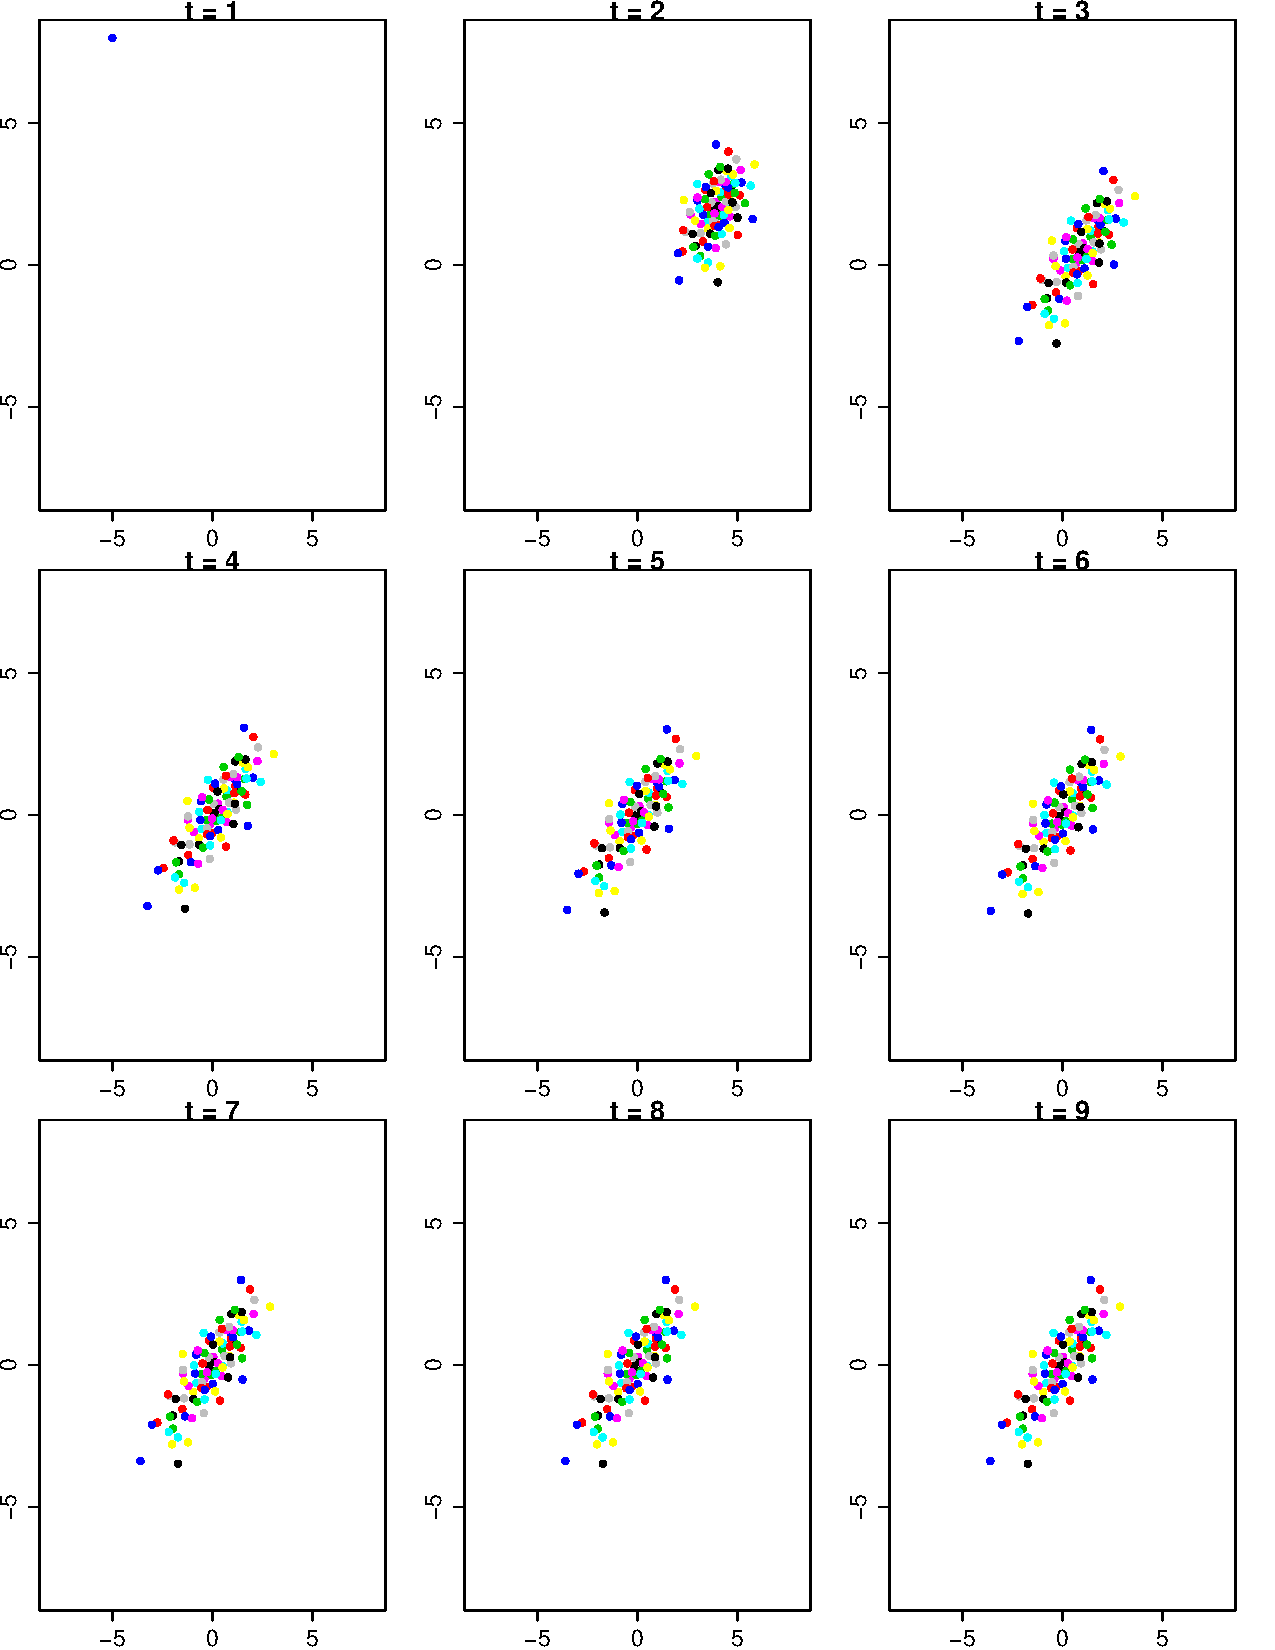
\includegraphics[scale = 0.8]{3b.pdf}
	\caption{Problem 3 - $X_0 = -5, Y_0 = 8, \rho = 0.5$} 
\end{figure}
\newpage
\begin{figure}[h!]
	\centering
	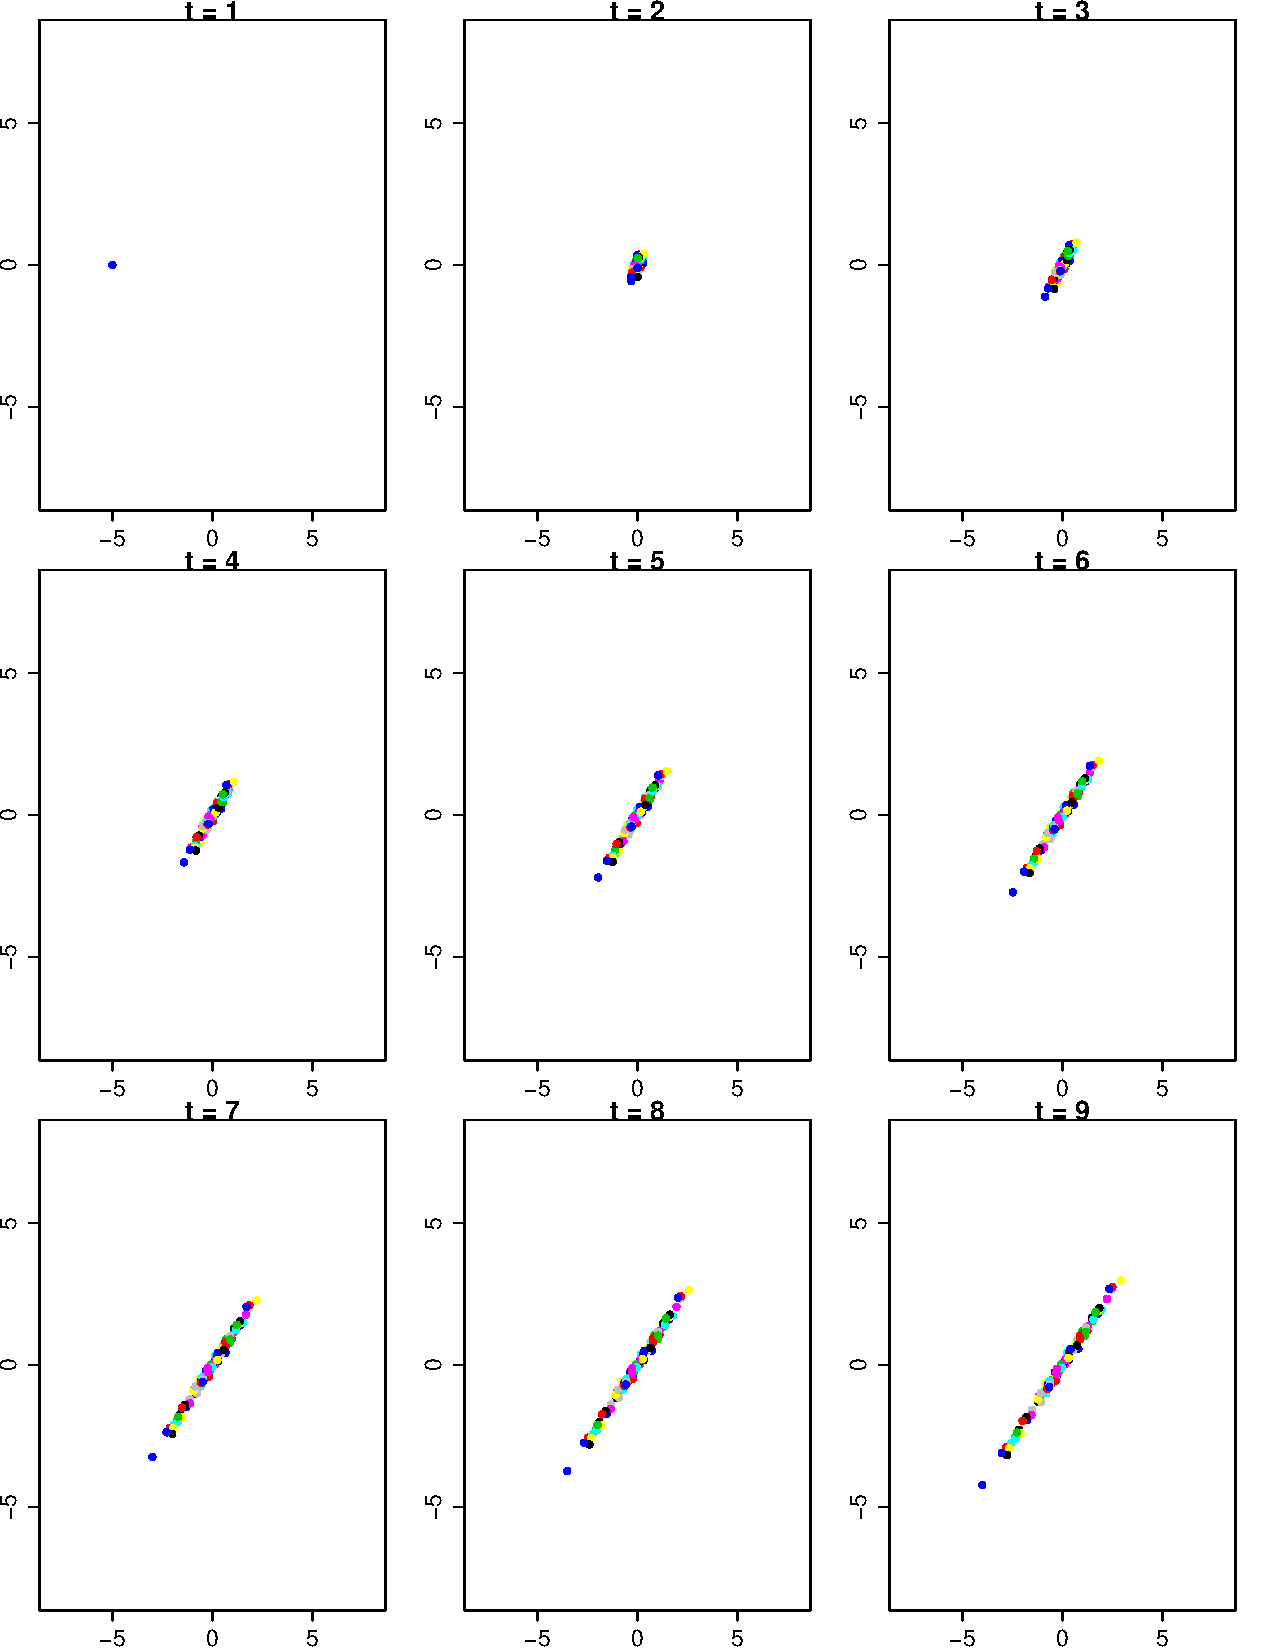
\includegraphics[scale = 0.8]{3c.pdf}
	\caption{Problem 3 - $X_0 = 5, Y_0 = 0, \rho = 0.99$}
	
\end{figure}
\end{document}